\documentclass[a4paper]{article}
\usepackage[14pt]{extsizes}
\usepackage{amssymb}  %  Математические символы
\usepackage{amsmath}  %  Математический пакет
\usepackage{amsthm}  %  Пакет для использования теорем
\usepackage{caption}  %  Пакет для использования подписей
\usepackage{misccorr}  %  Пакет с большинством настроек русских типографических правил - точки после цифр в оглавлении, etc.
\usepackage[noadjust]{cite}
\usepackage{cmap} % Для возможности нормального поиска в тексте и копирования!
\usepackage[utf8]{inputenc}  %  Кодировка исходного файла, который я тут вижу
\usepackage[T2A]{fontenc}  %  Набор символов на выходе, T2A включает в себя кириллицу
\usepackage[german, english, russian]{babel}
\usepackage{graphics}
\usepackage{graphicx}
\usepackage{indentfirst}  %  Либо подключать этот пакет, либо писать каждый раз \indentfirst в начале каждой главы (на Западе не ставят первую красную строку)
\usepackage{verbatim}  %  Окружение для вставки raw-кода
\usepackage{makeidx}
\usepackage{geometry}  %  Настройка геометрии вёрстки -- например, полей
\usepackage{hyperref}
\usepackage{fancyvrb}
\usepackage{color} %% это для отображения цвета в коде
\usepackage{listings} %% собственно, это и есть пакет listings
\usepackage{wrapfig}
\usepackage{setspace}
\usepackage{mathabx}

\DeclareCaptionFont{white}{\color{white}} %% это сделает текст заголовка белым
\DeclareCaptionFormat{listing}{\colorbox{gray}{\parbox{\textwidth}{#1#2#3}}}
\captionsetup[lstlisting]{format=listing,labelfont=white,textfont=white}
\DeclareGraphicsExtensions{.pdf,.png,.jpg}

\geometry{pdftex, left = 2cm, right = 2cm, top = 2.5cm, bottom = 2.5cm}
\righthyphenmin = 2
\begin{document}
	\begin{titlepage}
		\centering
		\begin{wrapfigure}[7]{l}{0.14\linewidth}
			\vspace{5mm}
			\hspace{-5.8mm}
			
\includegraphics[width=0.93\linewidth]{gerb}
		\end{wrapfigure}
		{\singlespacing \footnotesize \bfseries Министерство науки и высшего образования Российской Федерации\\Федеральное государственное бюджетное образовательное учреждение\\высшего образования\\<<Московский государственный технический университет\\имени Н.~Э.~Баумана\\ (национальный исследовательский университет)>>\\(МГТУ им. Н.~Э.~Баумана)\\}
		
		\textbf {\bf \underline{\hspace{\linewidth}}}
		\doublespacing \small \raggedright ФАКУЛЬТЕТ \hspace{25mm} \underline { «Информатика и системы управления»}\\
		КАФЕДРА \hspace{5mm} \underline {«Программное обеспечение ЭВМ и информационные технологии»}\\
		
		\vspace{30mm}
		\begin{center}
		\textbf{Отчёт по лабораторной работе №3}\\
		{\bf	По дисциплине: <<Анализ алгоритмов>>}\\
		{\bf Тема:} \underline {<<Трудоемкость алгоритмов>>}\\
		\end{center}
		\begin{flushleft}
			{\bf Студент}  \underline{Мередова Айджахан}\underline {\hspace{7cm}}
			\newline
			{\bf Группа} \underline{ИУ7-56Б}\underline {\hspace{10cm}}
			\newline
			{\bf Преподаватели} \underline {Волкова Л.Л., Строганов Ю.В.}
		\end{flushleft}
		\vfill
		
		\centering Москва - 2020 г.\\
	\end{titlepage}
	\lstset{ %
		language=Python,                 % выбор языка для подсветки 
		basicstyle=\small\sffamily, % размер и начертание шрифта для подсветки кода
		%numbers=left,               % где поставить нумерацию строк (слева\справа)
		numberstyle=\tiny,           % размер шрифта для номеров строк
		stepnumber=1,                   % размер шага между двумя номерами строк
		numbersep=5pt,                % как далеко отстоят номера строк от подсвечиваемого кода
		backgroundcolor=\color{white}, % цвет фона подсветки - используем \usepackage{color}
		showspaces=false,            % показывать или нет пробелы специальными отступами
		showstringspaces=false,      % показывать или нет пробелы в строках
		showtabs=false,             % показывать или нет табуляцию в строках
		frame=single,              % рисовать рамку вокруг кода
		tabsize=2,                 % размер табуляции по умолчанию равен 2 пробелам
		captionpos=t,              % позиция заголовка вверху [t] или внизу [b] 
		breaklines=true,           % автоматически переносить строки (да\нет)
		breakatwhitespace=false, % переносить строки только если есть пробел
		escapeinside={\%*}{*)}   % если нужно добавить комментарии в коде
	}
	
	\section*{Введение}
	Под сортировкой обычно принимают процесс перестановки объектов некоторого множества в определенном порядке. Цель сортировки — облегчить в дальнейшем поиск элементов отсортированного множества. Это очень часто выполняемая, фундаментальная операция. Объекты сортируются в телефонных справочниках, в списках налогоплательшиков, в оглавлениях книг, в библиотеках,в словарях, на складах, то есть почти всюду, где нужно искать хранимые объекты. \\
	
	
	Целями данной лабораторной работы являются:
	\begin{enumerate}
		\item реализовать три различных алгоритма сортировки;
		\item теоретически вычислить эффективность алгоритмов;
		\item сравнить алгоритмы по времени;
	\end{enumerate}
	\clearpage
	
	\section{Аналитическая часть}
	Cортировка - весьма важная операция, особенно в обработке данных. Также она идеальная тема для демонстарции широкого разнообразия алгоритмов, решаюших одну и ту же задачу, причем многие из них в каком-нибудь смысле оптимальны, и почти из них имеет какие-нибудь преимущества перед остальными. Поэтомк здесь хорошо видно, зачем нужен анализ эффективности алгоритмов. Более того, на примере сортировок становится понятно, что можно получить весьма существенный выигрыш в эффективности, разрабатывая хитроумные алгоритмы, даже если уже имеются очевидные методы.
	
	\subsection{Описание задачи}
	Алгоритм сортировки - это алгоритм для упорядочивания элементов в списке. В случае, когда элемент списка имеет несколько полей, поле, служащее критерием порядка, называется ключом сортировки. На практике в качестве ключа часто выступает число, а в остальных полях хранятся какие-либо данные, никак не влияющие на работу алгоритма.
	
	\subsubsection{Сортировка пузырьком}
	Простая сортировка выбором, она же пузырьковая использует сравнение и обмен пар соседних элементов до тех пор, пока не будут отсортированы все элементы.
	
	Здесь выполняются повторные проходы по массиву, причем каждый раз наименьший элемент оставшегося множества просеивается в направлении левого конца массива. Если для разнообразия считать массив расположенным вертикально, а не горизонтально, и вообразить, что элементы - это пузырьки в сосуде с водой, причем их вес равен значению ключа, тогда проходы по массиву приводят к подъему пузырька на уровень, соответствующий его весу. Отсюда и название этого алгоритма сортировки.
	
	\textbf{Сложность по времени:}
	\begin{itemize}
	\item худший случай (элементы массива отсортированы в обратном порядке): O($n^{2}$) 
	\item средний случай (рандомное расположение элементов массива): О$(n^{2}$)
	\item лучший случай (массив отсортирован): O($n$)
	\end{itemize}

	\subsubsection{Шейкер-сортировка}
	Этот алгоритм является улучшенной версией пузырьковой сортировки. Можно встретить другие  названия этой сортировки: сортировка перемешиванием, пульсирующая сортировка, двунаправленная сортировка пузырьком.
	
	Этот алгоритм сортировки отличается от пузырьковой тем, что она двунаправленная: алгоритм перемещается не строго слева направо, а сначала слева направо, затем справа налево.
	Шейкер-сортировка выгодна в тех случаях, когда элементы уже стоят в почти правильном порядке, - но это редко случается на практике.
	\textbf{Сложность по времени:}
	\begin{itemize}
		\item худший случай (элементы массива отсортированы в обратном порядке): O($n^{2}$) 
		\item средний случай (рандомное расположение элементов массива): О$(n^{2}$)
		\item лучший случай (массив отсортирован): O($n$)
	\end{itemize}


	\subsubsection{Сортировка Шелла}
	В 1959 г. Шелл предложил ускорить сортировку простыми вставками. 
	
	В этом алгоритме очень остроумный подход в определении того, какую именно часть массива считать отсортированной. В простых вставках все просто: от текущего элемента всё что слева — уже отсортировано, всё что справа — ещё не отсортировано. В отличие от простых вставок сортировка Шелла не пытается слева от элемента сразу формировать строго отсортированную часть массива. Она создаёт слева от элемента почти отсортированную часть массива и делает это достаточно быстро.
	
	Сортировка Шелла закидывает текущий элемент в буфер и сравнивает его с левой частью массива. Если находит бoльшие элементы слева, то сдвигает их вправо, освобождая место для вставки. Но при этом берёт не всю левую часть, а только некоторую группу элементов из неё, где элементы разнесены друг от друга на некоторое расстояние. Такая система позволяет быстро вставлять элементы примерно в ту область массива, где они должны находиться.
	
	С каждой итерацией основного цикла это расстояние постепенно уменьшается и когда оно становится равным единице, то сортировка Шелла в этот момент превращается в классическую сортировку простыми вставками, которой дали на обработку почти отсортированный массив. А почти отсортированный массив сортировка вставками в полностью отсортированный преобразует быстро.
	\clearpage
	
	\textbf{Сложность по времени:}
	\begin{itemize}
		\item худший случай (если неправильно выбраны промежутки): O($n (log_{n})^{2}$) 
		\item средний случай (рандомное расположение элементов массива):O($n (log_{n})^{2}$) или $n^{3/2}$
		\item лучший случай (массив отсортирован): O($n$)
	\end{itemize}

	\section{Конструкторская часть}
	Рассмотрим сортироку пузырьком, шейкер-сортировку и сортировку Шелла.
	
	\subsection{Схемы алгоритмов}
	На рисунке ~\ref{image1} изображена схема алгоритма сортировки пузырьком.
	 \begin{figure}[h]
		\center{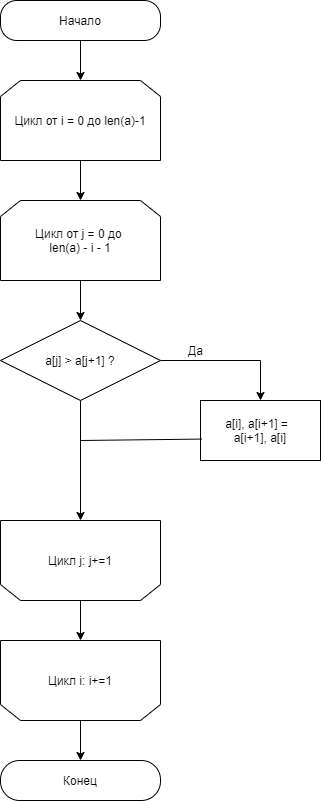
\includegraphics[width=0.5\linewidth, height = 0.5\textheight]{bubblesort}}
		\caption{Схема алгоритма сортировки пузырьком. \centering}
		\label{image1}
	\end{figure}
	\clearpage
	
	На рисунках ~\ref{image2} - ~\ref{image3} изображены схемы алгоритма шейкер-сортировки.
	\begin{figure}[h]
		\center{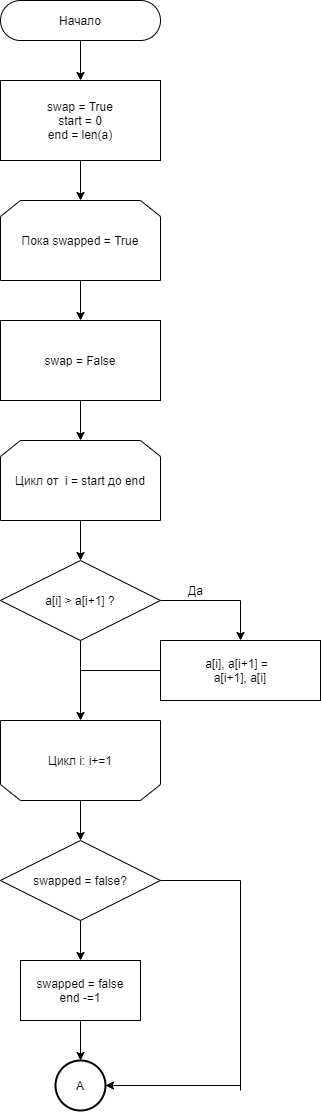
\includegraphics[width=0.5\linewidth, height = 0.5\textheight]{shaker1}}
		\caption{Схема алгоритма шейкер - сортировки(1). \centering}
		\label{image2}
	\end{figure}

		
	\begin{figure}[h]
		\center{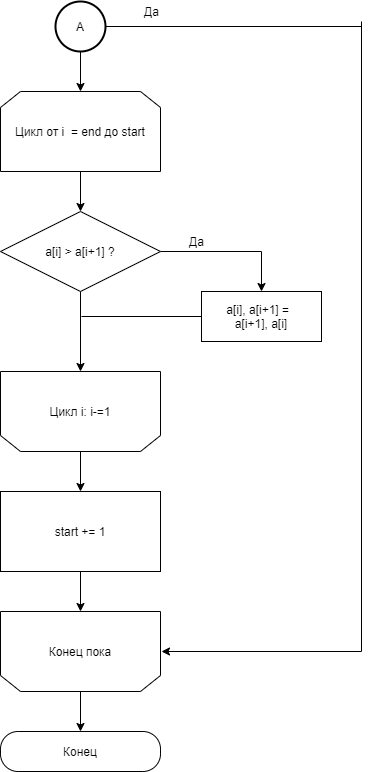
\includegraphics[width=0.5\linewidth, height = 0.5\textheight]{shaker2}}
		\caption{Схема алгоритма шейкер - сортировки(2). \centering}
		\label{image3}
	\end{figure}	
	
	
	\begin{figure}[h]
		\center{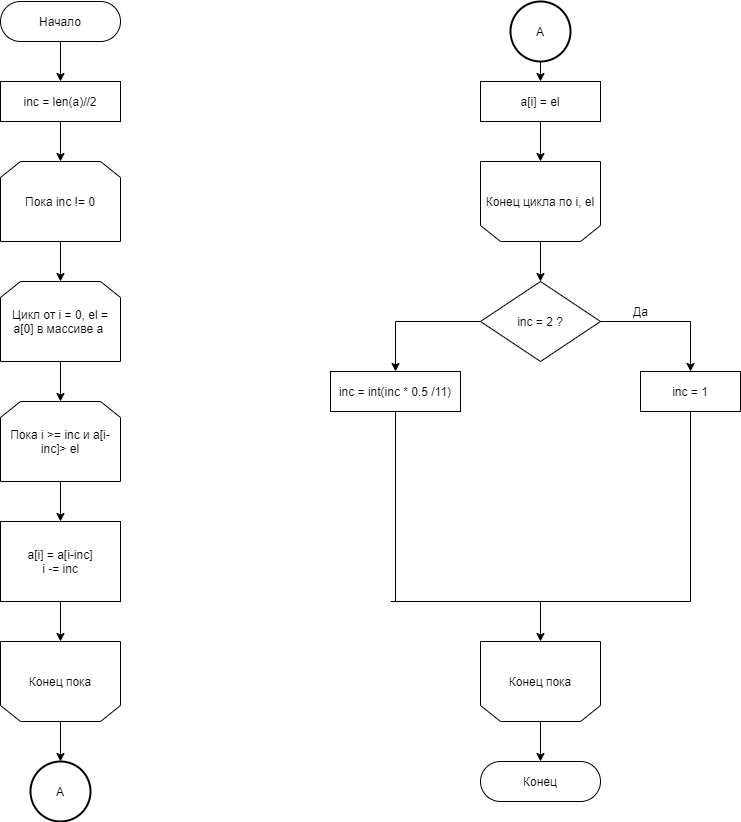
\includegraphics[width=0.8\linewidth, height = 0.8\textheight]{shell}}
		\caption{Схема алгоритма сортировки Шелла (2). \centering}
		\label{image4}
	\end{figure}	
	\clearpage
	
	
	\section{Технологическая часть}
	\subsection{Требования к программному обеспечению}
	Программное обеспечение должно обеспечивать замер процессорного времени выполнения каждого алгоритма. Проводятся замеры для случайно генерируемых массивов размерности до 10000.
	
	\subsection{Средства реализации}
	Python\cite{what_is_python} — это высокоуровневый язык программирования, который используется в различных сферах IT, таких как машинное обучение, разработка приложений, web, парсинг и другие.
	С ним легко работать, что сокращает время разработки. Написанный в удобочитаемом формате, Python делает процесс разработки программного обеспечения быстрым, удобным и максимально упрощенным.
	По сравнению с другими языками, Python в 5-10 раз быстрее по времени разработки, однако медленный при выполнении программ. Он обеспечивает расширенные возможности управления процессами и объектно-ориентированный дизайн, помогая как в скорости, так и в производительности.
	\clearpage
	
	\subsection{Методы замера времени в программе}
	\subsubsection{Время}
	Сушествует несколько способов измерения процессорного времени исполнения программы. 
	Помимо стандратного модуля $time$ есть библиотека $timeit$ \cite{timeit}. Этот модуль предоставляет простой способ найти время выполнения маленьких битов кода Python.
	$timeit$ запускает фрагмент кода миллионы раз(значение по умолчанию - 1000000), так что получаем наиболее статистически значимое измерение времени выполнения кода.
	
	\subsubsection{Улучшение точности замеров времени} Чтобы получить более точные результаты, каждый тест запускается несколько раз, все полученные значения времени(в тиках) суммируются и делятся на количество запусков кода. Таким образом, получаем среднее время выполнения кода.
	\clearpage
	\subsection{Листинг кода}
	
	\begin{lstlisting}[label = bubble, caption = Сортировка пузырьком]
		def bubbleSort(data):
			N = len(data)
			for i in range(N-1):
				for j in range(N-i-1):
					if data[j] > data[j+1]:
						data[j], data[j+1] = data[j+1], data[j]
		
		
	\end{lstlisting}

	
	\begin{lstlisting}[label = shaker, caption = Шейкер-сортировка]
def cocktailSort(array): 
	length = len(array) 
	swapped = True
	start_index = 0
	end_index = length - 1
	
	while (swapped == True): 
		swapped = False
		# prohod sleva naprovo
		for i in range(start_index, end_index): 
			if (array[i] > array[i + 1]) : 
			# obmen elementov
				array[i], array[i + 1] = array[i + 1], array[i] 
				swapped = True
	
		# yesli ne bylo obmenov break
		if (not(swapped)): 
			break
	
		swapped = False
		end_index = end_index - 1
	
		# prohod sprava nalevo
		for i in range(end_index - 1, start_index - 1, -1): 
			if (array[i] > array[i + 1]): 
			# obmen
				array[i], array[i + 1] = array[i + 1], array[i] 
				swapped = True
	
		start_index = start_index + 1
	
	\end{lstlisting}


	\begin{lstlisting}[label = shell, caption = Сортировка Шелла]
	def shellSort(data):
		inc = len(data) // 2
		while inc:
			for i, el in enumerate(data):
				while i >= inc and data[i - inc] > el:
					data[i] = data[i - inc]
					i -= inc
				data[i] = el
			inc = 1 if inc == 2 else int(inc * 5.0 / 11)
	\end{lstlisting}
	\clearpage
	\section{Экспериментальная часть}
	Проведём тестирование сравним алгоритмы по времени работы.
	
	\subsection{Примеры работ}
	
	Ниже приведены примеры работ.
	
	\begin{lstlisting}[label = ex1, caption = Пример работы алгоритмов на сортированный массив]
	Source array:  [-187, -88, 26, 52, 110, 164]
	Expected array:  [-187, -88, 26, 52, 110, 164]
	Bubble Sort:  [-187, -88, 26, 52, 110, 164]
	Shell Sort:  [-187, -88, 26, 52, 110, 164]
	Shaker Sort:  [-187, -88, 26, 52, 110, 164]
	\end{lstlisting}
	
	
	
	\begin{lstlisting}[label = ex2, caption = Пример работы алгоритмов на случайный массив]
	Source array:  [-136, -18, 146, 116, -64, -91]
	Expected array:  [-136, -91, -64, -18, 116, 146]
	Bubble Sort:   [-136, -91, -64, -18, 116, 146]
	Shell Sort:  [-136, -91, -64, -18, 116, 146]
	Shaker Sort:  [-136, -91, -64, -18, 116, 146]
	\end{lstlisting}



	\begin{lstlisting}[label = ex3, caption = Пример работы алгоритмов на обратно отсортированный массив]
	Source array:  [177, 133, 82, 50, 46, -189]
	Expected array:  [-189, 46, 50, 82, 133, 177]
	Bubble Sort:   [-189, 46, 50, 82, 133, 177]
	Shell Sort:  [-189, 46, 50, 82, 133, 177]
	Shaker Sort:  [-189, 46, 50, 82, 133, 177]
	\end{lstlisting}



	\begin{lstlisting}[label = ex4, caption = Пример работы алгоритмов массив с одинаковыми элементами]
	Source array:  [5, 5, 5, 5, 5, 5]
	Expected array:  [5, 5, 5, 5, 5, 5]
	Bubble Sort:   [5, 5, 5, 5, 5, 5]
	Shell Sort:  [5, 5, 5, 5, 5, 5]
	Shaker Sort:  [5, 5, 5, 5, 5, 5]
	\end{lstlisting}

	Все тесты прошли успешно.
	\clearpage
	
	\subsection {Замеры времени}
	Ниже в таблице ~\ref{table1} представлены результаты замера времени для отсортированного массива, в таблице ~\ref{table2} - для обратно отсортированного массива и в таблице ~\ref{table3} - для случайно сгенерированного массива.
	\begin{table}[h]
		\caption{\label{table1} Результаты замера времени для отсортированного массива.}
		\begin{center}
			\begin{tabular}{|p{200pt}|p{50pt}|p{50pt}|p{50pt}|p{50pt} |p{50pt}|}
				\hline
				\textbf{Алгоритм} & \textbf{100} & \textbf{300} &\textbf{500} & \textbf{700} & \textbf{1000}\\ \hline
				Сортировка пузырьком & 77603 & 433224  & 1199938 &2562328 & 5016702\\	\hline
				Шейкер-сортировка & 2137 & 2854 & 7722 & 7089 & 12066\\ \hline
				Сортировка Шелла & 8437 & 34295 & 57884 & 95701 & 149729\\ \hline
			\end{tabular}
		\end{center}
	\end{table}\\
	\begin{table}[h]
	\caption{\label{table2} Результаты замера времени для обратно отсортированного массива.}
	\begin{center}
		\begin{tabular}{|p{200pt}|p{50pt}|p{50pt}|p{50pt}|p{50pt} |p{50pt}|}
			\hline
			\textbf{Алгоритм} & \textbf{100} & \textbf{300} &\textbf{500} & \textbf{700} & \textbf{1000}\\ \hline
			Сортировка пузырьком &56473 & 477015  & 1386094 & 2862636 & 5539335 \\	\hline
			Шейкер-сортировка & 11633 &107924 & 362706 & 635177 &  1343340\\ \hline
			Сортировка Шелла & 7352 & 35593 & 69416 &114963 & 137485\\ \hline
		\end{tabular}
	\end{center}
\end{table}\\

\begin{table}[h]
	\caption{\label{table3} Результаты замера времени для случайно сгенерированного массива.}
	\begin{center}
		\begin{tabular}{|p{200pt}|p{50pt}|p{50pt}|p{50pt}|p{50pt} |p{50pt}|}
			\hline
			\textbf{Алгоритм} & \textbf{100} & \textbf{300} &\textbf{500} & \textbf{700} & \textbf{1000}\\ \hline
			Сортировка пузырьком & 71631 & 500447 & 1310741 & 2577064 & 5378399 \\	\hline
			Шейкер-сортировка & 7308 &86722 & 262657 & 460562 &  942419\\ \hline
			Сортировка Шелла & 8068 & 40303 & 121758 &128520 & 142852\\ \hline
		\end{tabular}
	\end{center}
\end{table}

\clearpage

\subsection{Выводы}
Из результатов замер времени алгоритмов сортировки можно сделать следующие выводы:
\begin{enumerate}
	\item сортировка пузырьком работет медленее, чем сортировка Шелла и Шейкер-сортировка;
	\item у алгоритма сортировки Шелла при обратно отсортированном массиве самые лучшие результаты по времени выполнения;
	\item Шейкер-сортировка выгодна в тех случаях, когда элементы уже стоят почти в правильном порядке, - но это случается редко на практике.\cite{nikvirt}
\end{enumerate}
\clearpage

\subsection{Графики}
\begin{figure}[h]
	\center{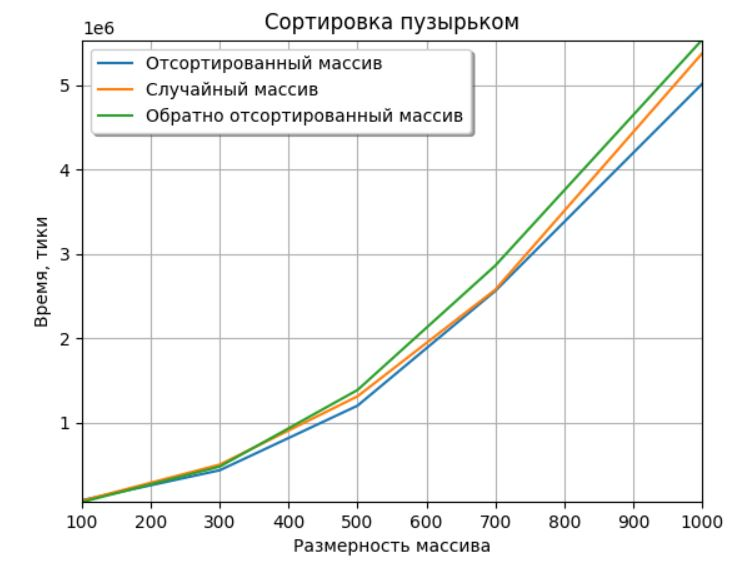
\includegraphics[width=0.8\linewidth, height = 0.5\textheight]{bubble}}
	\caption{График зависимости времени алгоритма сортировки пузырька. \centering}
	\label{image5}
\end{figure}

\begin{figure}[h]
	\center{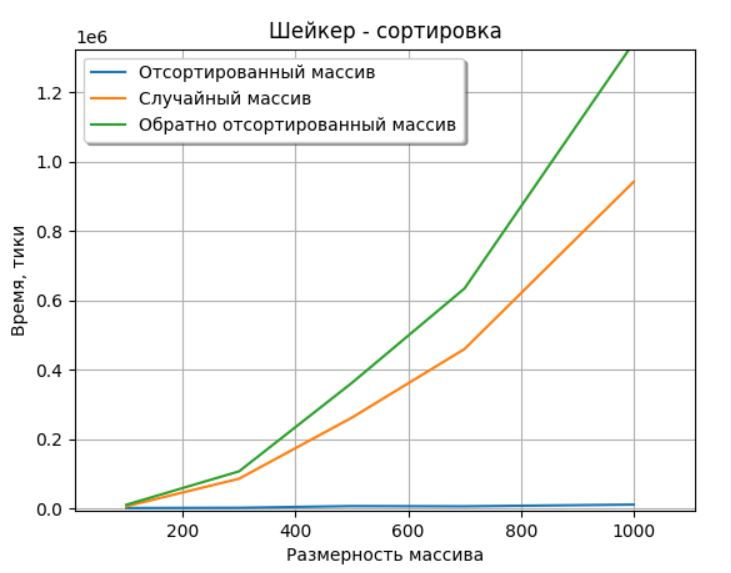
\includegraphics[width=0.8\linewidth, height = 0.5\textheight]{shaker}}
	\caption{График зависимости времени алгоритма Шейкер-сортировки. \centering}
	\label{image6}
\end{figure}

\begin{figure}[h]
	\center{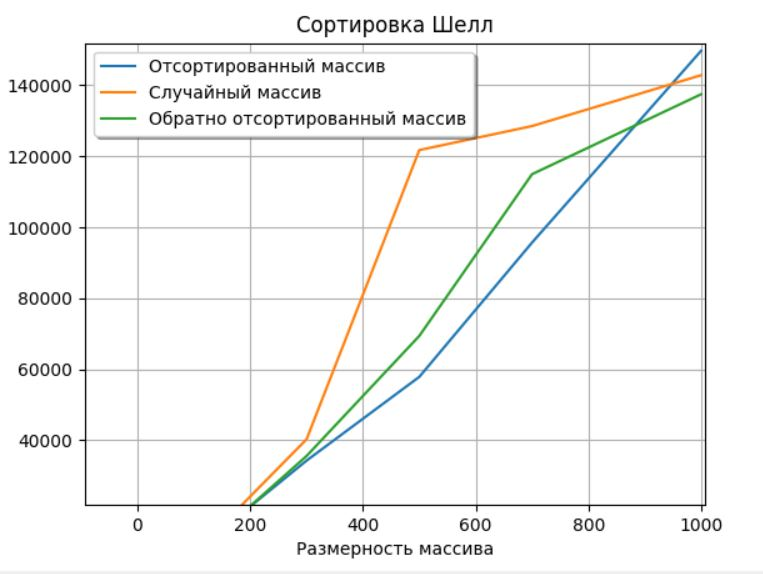
\includegraphics[width=0.8\linewidth, height = 0.5\textheight]{shell_gr}}
	\caption{График зависимости времени алгоритма сортировки Шелла. \centering}
	\label{image7}
\end{figure}
\clearpage

\section{Заключение}
В ходе данной работы было проведено сравнение трех алгоритмов сортировки массива: сортировка пузырьком, Шейкер-сортировка, сортировка Шелла.

Были сделаны следуюшие выводы:
\begin{enumerate}
	\item сортировка пузырьком работет медленее, чем сортировка Шелла и Шейкер-сортировка;
	\item у алгоритма сортировки Шелла при обратно отсортированном массиве самые лучшие результаты по времени выполнения;
	\item Шейкер-сортировка выгодна в тех случаях, когда элементы уже стоят почти в правильном порядке, - но это случается редко на практике. \cite{nikvirt}
\end{enumerate}
Из рассмотренных трех алгоритмов самым лучшим алгоритмом сортировки является сортировка Шелла.
\clearpage

	\begin{thebibliography}{6}
	\bibitem{what_is_python}	 
	Python:что нужно знать. [ЭЛ. РЕСУРС]\\
	Режим доступа: https://skillbox.ru/media/code/story\_buzunov/ \\
	(Дата обращения: 10.11.2020)
	\bibitem{timeit}
	Timeit в Python с примерами. [ЭЛ. РЕСУРС]\\
	Режим доступа: http://espressocode.top/timeit-python-examples/ \\
	(Дата обращения: 10.11.2020)
	\bibitem {nikvirt}
	\label{virt}
	Никлаус Вирт Алгоритмы и структуры данных. Новая версия для Обертона/Пер. с англ. Ткачев Ф.В. --  М.:ДМК Пресс, 2016--272 с.:ил.\\
	(Дата обращения: 10.11.20)\\
	\bibitem {shaker}
	\label{shakersort}
	Шейкерная сортировка [ЭЛ. РЕСУРС] \\
	Режим доступа: https://purecodecpp.com/archives/1895 \\
	(Дата обращения: 10.11.20)\\
	
	\bibitem {insert}
	Сортировки вставками [ЭЛ.РЕСУРС] \\
	Режим доступа: https://habr.com/ru/post/415935/ \\
	(Дата обращения: 10.11.20)\\
	
	\bibitem{bubble}
	Пузырьковая сортировкаи все-все-все [ЭЛ.РЕСУРС] \\
	Режим доступа: https://habr.com/ru/post/204600/ \\
	(Дата обращения: 10.11.20)\\
\end{thebibliography}



	
	

\end{document}